\documentclass[aps,prc,reprint,nobalancelastpage]{revtex4-1}

\usepackage{siunitx}
\usepackage{amsmath}
\usepackage{mathtools}
\usepackage{algorithm}
\usepackage{algpseudocode}
% \usepackage{minted}
\usepackage{url}
\frenchspacing

\newcommand{\sun}[0]{\ensuremath{\odot}}

% \usemintedstyle{xcode}


\begin{document}

\title{Project 3: A model of the solar system}
\author{Joshua Bradt}
\noaffiliation
\date{April 1, 2016}

\maketitle

\section{Introduction}
\label{sec:introduction}

    The solar system is a simple, physically meaningful system to use when comparing different techniques for solving differential equations. Using Newtonian gravity (and ignoring relativistic effects), the planets are held in orbit around the sun by the inverse square law force
    \begin{equation}
        \mathbf{F} = \frac{G m_1 m_2}{r^3} \mathbf{r}.
    \end{equation}
    Here, the vector $\mathbf{r}$ points from one body to the other.

    For $N$ bodies, this generalizes to give the following force on body $k$:
    \begin{equation}
        \mathbf{F}_k = \sum_{i \neq k} \frac{G m_i m_k}{r_{ik}^3} \mathbf{r}_{ik}
    \end{equation}
    Naturally there are $N$ such equations for the $N$ bodies in the system. In Cartesian coordinates, these can be rewritten as $3N$ coupled equations:
    \begin{align}
        \frac{d^2 x_k}{dt^2} &= \sum_{i \neq k} \frac{G m_i}{r_{ik}^3} (x_i - x_k) \\
        \frac{d^2 y_k}{dt^2} &= \sum_{i \neq k} \frac{G m_i}{r_{ik}^3} (y_i - y_k) \\
        \frac{d^2 z_k}{dt^2} &= \sum_{i \neq k} \frac{G m_i}{r_{ik}^3} (z_i - z_k)
    \end{align}
    where
    \begin{equation}
        r_{ik} = \sqrt{(x_i - x_k)^2 + (y_i - y_k)^2 + (z_i - z_k)}.
    \end{equation}
    The motion of the planets can then be simulated given appropriate initial conditions and an algorithm for solving these equations.

\section{Numerical algorithms}
\label{sec:algorithms}

    \subsection{Euler's method}
    \label{sub:euler}

        Perhaps the simplest method for solving a set of differential equations is Euler's method. This simple algorithm uses the first derivatives to step from one point to the next.

        Given an initial position $\mathbf{r}_i$ and velocity $\mathbf{v}_i$ at time $t_i$, the position and the velocity at the next step are calculated as
        \begin{align}
            \mathbf{v}_{i+1} &= \mathbf{v}_i + \frac{\mathbf{F}(\mathbf{r}_i, t_i)}{m_i} \Delta t \\
            \mathbf{r}_{i+1} &= \mathbf{r}_i + \mathbf{v}_i \Delta t
        \end{align}

        This algorithm is very simple to implement, but as a first-order method, its $O(\Delta t)$ error can severely limit the precision of the results. This can be helped by choosing a small time step, but this increases computation time.

        % \begin{figure}
            \begin{algorithm}[H]
                \begin{algorithmic}
                    \Function{Euler}{$\mathbf{r}$, $\mathbf{v}$, $h$}
                        \State $\mathbf{a} \gets \text{findAcceleration}(\mathbf{r})$
                        \State $\mathbf{v}' \gets \mathbf{v} + h \mathbf{a}$
                        \State $\mathbf{r}' \gets \mathbf{r} + h \mathbf{v}$
                        \State \textbf{return} $(\mathbf{r}', \mathbf{v}')$
                    \EndFunction
                \end{algorithmic}
                \caption{Euler method for position and velocity}
            \end{algorithm}
        % \end{figure}

    \subsection{Velocity Verlet algorithm}
    \label{sub:verlet}

        Another method for solving the equations can be found by beginning with Taylor expansions for the position and velocity:
        \begin{align}
            \mathbf{r}(t+h) &= \mathbf{r}(t) + h \dot{\mathbf{r}}(t) + \frac{h^2}{2}\ddot{\mathbf{r}}(t) + O(h^3) \label{eq:verletp}\\
            \mathbf{v}(t+h) &= \mathbf{v}(t) + h \dot{\mathbf{v}}(t) + \frac{h^2}{2}\ddot{\mathbf{v}}(t) + O(h^3). \label{eq:verletv}
        \end{align}
        To second order, the derivative of the second equation is
        \begin{equation}
            \dot{\mathbf{v}}(t+h) = \dot{\mathbf{v}}(t) + h \ddot{\mathbf{v}}(t) + O(h^2)
        \end{equation}
        which can be rearranged to find:
        \begin{equation}
            \frac{h^2}{2}\ddot{\mathbf{v}}(t) = \frac{h}{2} [\dot{\mathbf{v}}(t+h) - \dot{\mathbf{v}}(t)] + O(h^3).
        \end{equation}
        This can then be plugged into (\ref{eq:verletv}) to find
        \begin{equation}
            \mathbf{v}(t+h) = \mathbf{v}(t) + \frac{h}{2} [\dot{\mathbf{v}}(t+h) + \dot{\mathbf{v}}(t)] + O(h^3).
        \end{equation}
        Finally, note that $\mathbf{v}(t) = \dot{\mathbf{r}}(t)$ and $\mathbf{F}(t) = \dot{\mathbf{v}}(t) = \ddot{\mathbf{r}}(t)$, so (\ref{eq:verletp}) and (\ref{eq:verletv}) can be rewritten (in discretized form) as
        \begin{gather}
            \mathbf{r}_{i+1} = \mathbf{r}_i + h\mathbf{v}_i + \frac{h^2}{2} \frac{\mathbf{F}(\mathbf{r}_i, t_i)}{m} + O(h^3) \\
            \mathbf{v}_{i+1} = \mathbf{v}_i + \frac{h}{2} \left(\frac{\mathbf{F}(\mathbf{r}_{i+1}, t_{i+1})}{m} + \frac{\mathbf{F}(\mathbf{r}_i, t_i)}{m}\right) + O(h^3)
        \end{gather}
        These two equations can then be evaluated in the order written at each iteration to find the new position and velocity for each body.

        % \begin{figure}
            \begin{algorithm}[H]
                \begin{algorithmic}
                    \Function{Verlet}{$\mathbf{r}$, $\mathbf{v}$, $h$}
                        \State $\mathbf{a} \gets \text{findAcceleration}(\mathbf{r})$
                        \State $\mathbf{r}' \gets \mathbf{r} + h \mathbf{v} + \frac{1}{2} h^2 \mathbf{a}$
                        \State $\mathbf{a}' \gets \text{findAcceleration}(\mathbf{r}')$
                        \State $\mathbf{v}' \gets \mathbf{v} + \frac{1}{2} h (\mathbf{a} + \mathbf{a}')$
                        \State \textbf{return} $(\mathbf{r}', \mathbf{v}')$
                    \EndFunction
                \end{algorithmic}
                \caption{Verlet method for position and velocity}
            \end{algorithm}
        % \end{figure}

    \subsection{Runge-Kutta method}
    \label{sub:rk4}

        The final method that will be considered here is the fourth-order Runge-Kutta method, or RK4. This method of numerical integration is similar to Simpson's rule, which states that
        \begin{equation*}
            \int_{a}^{b} f(x)\,dx \approx \frac{b-a}{6} \left( f(a) + 4 f\!\left(\frac{a+b}{2}\right) + f(b) \right)
        \end{equation*}
        In this case, the value of the function being integrated is known at the starting point but unknown at the midpoint and the end of the step. At these locations, the function is approximated using Euler's method. This leads to the set of equations
        \begin{align}
            k_1     &= f(x_i, t_i) \\
            k_2     &= f(x_i + \tfrac{h}{2} k_1, t_i + \tfrac{h}{2}) \\
            k_3     &= f(x_i + \tfrac{h}{2} k_2, t_i + \tfrac{h}{2}) \\
            k_4     &= f(x_i + h k_3, t_i + h) \\
            x_{i+1} &= x_i + \tfrac{h}{6}(k_1 + 2k_2 + 2k_3 + k_4) + O(h^5).
        \end{align}
        One clear advantage of this method is that the error scales as $h^5$, making this a much higher-order method than either of the previous two.

        % \begin{figure}[H]
            \begin{algorithm}[H]
                \begin{algorithmic}
                    \Function{RK4}{$\mathbf{r}$, $\mathbf{v}$, $h$}
                        \State $\mathbf{k}_1^v \gets \text{findAcceleration}(\mathbf{r})$
                        \State $\mathbf{k}_1^r \gets \mathbf{v}$
                        \State $\mathbf{k}_2^v \gets \text{findAcceleration}(\mathbf{r} + \frac{h}{2}\mathbf{k}_1^r)$
                        \State $\mathbf{k}_2^r \gets \mathbf{v} + \frac{h}{2} \mathbf{k}_1^v$
                        \State $\mathbf{k}_3^v \gets \text{findAcceleration}(\mathbf{r} + \frac{h}{2}\mathbf{k}_2^r)$
                        \State $\mathbf{k}_3^r \gets \mathbf{v} + \frac{h}{2} \mathbf{k}_2^v$
                        \State $\mathbf{k}_4^v \gets \text{findAcceleration}(\mathbf{r} + h\mathbf{k}_3^r)$
                        \State $\mathbf{k}_4^r \gets \mathbf{v} + h \mathbf{k}_3^v$
                        \State $\mathbf{v}' \gets \mathbf{v} + \frac{h}{6} (\mathbf{k}_1^v + 2\mathbf{k}_2^v + 2\mathbf{k}_3^v + \mathbf{k}_4^v)$
                        \State $\mathbf{r}' \gets \mathbf{r} + \frac{h}{6} (\mathbf{k}_1^r + 2\mathbf{k}_2^r + 2\mathbf{k}_3^r + \mathbf{k}_4^r)$
                        \State \textbf{return} $(\mathbf{r}', \mathbf{v}')$
                    \EndFunction
                \end{algorithmic}
                \caption{RK4 method for position and velocity}
            \end{algorithm}
        % \end{figure}

\section{Results}
\label{sec:results}

    The algorithms described above were implemented in a C++ program to track the motion of the planets. This code was run for a variety of test cases, which will be described in the following sections.

    \subsection{Earth-Sun system}
    \label{sub:earthsun}

        First, the code was tested considering only the motion of the Earth around the Sun. In this case, the orbit of the Earth was assumed to be circular, and the Sun was fixed in place at the origin of the two-dimensional coordinate system.

        The initial position of the Earth was set to the vector $\mathbf{r} = (\SI{1}{au}, \SI{0}{au})$ since \SI{1}{au} is defined as the approximate distance between the Earth and the Sun. The initial velocity of the Earth can then be found by equating the centripetal force to the gravitational force to find
        \begin{equation}
            v = \sqrt{\frac{G m_\sun}{r}} = \SI{1.7202e-2}{au/d}
        \end{equation}
        in the tangential direction, which is $y$ in this case. One result of running with these parameters is shown in Figure~\ref{fig:earthrk4}.

        \begin{figure}
            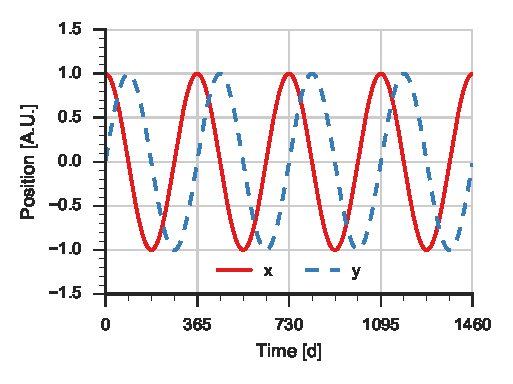
\includegraphics{earthpos_rk4.pdf}
            \caption{Earth's position over 4 years assuming a circular orbit. This was calculated using the RK4 integrator with a time step of \SI{1.0}{d}.}
            \label{fig:earthrk4}
        \end{figure}

        One test of the quality of this calculation is to check that the Earth's kinetic and potential energies and its angular momentum are constants. These must all be constant since for a circular orbit, the Earth-Sun distance and the Earth's velocity must remain constant. For the case shown in Figure~\ref{fig:earthrk4}, where the integration was done using the RK4 algorithm with a step size of \SI{1.0}{d}, the maximum deviation of the Earth's kinetic energy from its initial value was \SI{0.012}{\percent}, and the maximum deviation of the Earth-Sun distance from its initial value was \SI{0.0060}{\percent}. This implies that the kinetic energy, potential energy, and angular momentum were all constant.

        Due to its very small error of $O(h^5)$, RK4 will generally give good results for a reasonable step size, as shown above. On the other hand, the Euler method, using the same step size of \SI{1.0}{d}, produces a maximum kinetic energy deviation of \SI{1.76}{\percent} and a maximum deviation in the Earth-Sun distance of \SI{0.89}{\percent}. Even with a step size of \SI{0.01}{d}, these two deviations are larger than the RK4 values at \SI{0.024}{\percent} and \SI{0.012}{\percent}. This confirms that the choice of algorithm is very important when precise results are needed.

    \subsection{Escape velocity}
    \label{sub:escape}

        Another simple test is to plot the behavior of a planet at its escape velocity. The escape velocity is the velocity at which the planet's kinetic and potential energy are equal, or
        \begin{equation}
            v = \sqrt{\frac{2Gm_\sun}{r}} = \SI{2.4327e-2}{au/d}
        \end{equation}
        in the tangential direction. The results of running the program with this velocity are shown in Figure~\ref{fig:escape}.

        \begin{figure}
            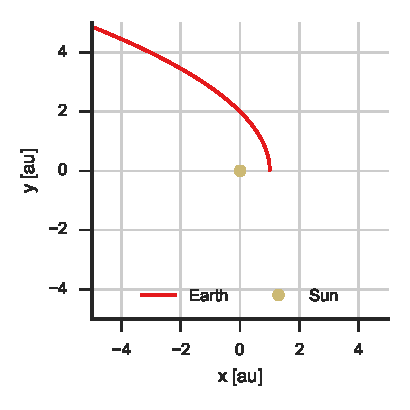
\includegraphics{escape.pdf}
            \caption{Trajectory of the Earth given an initial tangential velocity equal to its escape velocity. The trajectory appears to be parabolic, as expected. The step size was \SI{1.0}{d}, and the integrator was RK4.}
            \label{fig:escape}
        \end{figure}

    \subsection{Earth-Sun-Jupiter system}
    \label{sub:jupiter}

        To look at the stability of the Earth-Sun system, we can add an additional planet. The planet with the largest ability to perturb Earth's orbit is Jupiter, the most massive planet in the solar system at $m_J = \num{9.5458e-4}{m_\sun}$.

        As a first approximation, we will place Jupiter in a circular orbit at \SI{5.20}{au}, its mean distance from the Sun. Its initial position vector is $\mathbf{r} = (5.20, 0) \,\si{au}$ and its initial velocity vector is $\mathbf{v} = (0, \num{7.543e-3})\,\si{au/d}$.

        \begin{figure}
            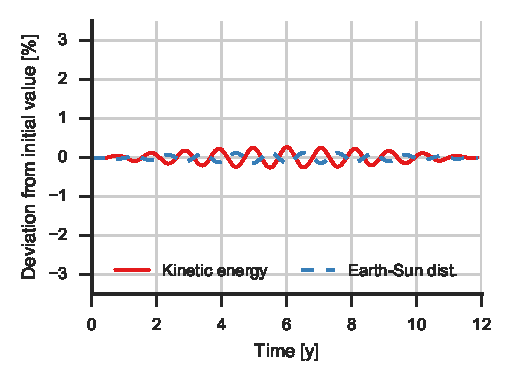
\includegraphics{jupiter_devs_1x.pdf}
            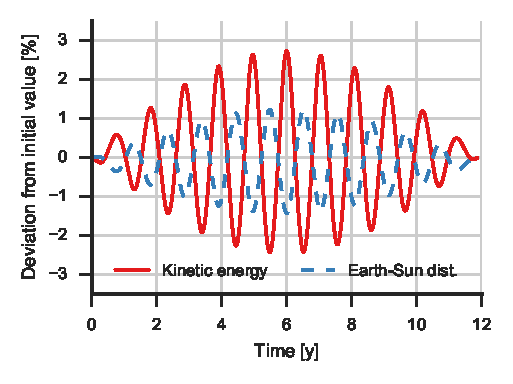
\includegraphics{jupiter_devs_10x.pdf}
            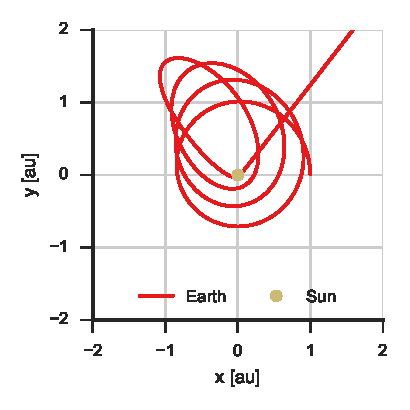
\includegraphics{jupiter_1000x.pdf}
            \caption{The effects of Jupiter on the Earth's orbit. Top: deviations in the Earth's kinetic energy and distance from the Sun for a normal-mass Jupiter. Middle: same as top, but with the mass of Jupiter multiplied by 10. Bottom: The trajectory of the Earth if the mass of Jupiter were 1000 times larger than normal. All of these were calculated with RK4 and a step size of \SI{1.0}{d}.}
            \label{fig:jupiter}
        \end{figure}

        The addition of Jupiter to the system influences the Earth's orbit and deforms it from the expected circular shape. This effect is greater if the mass of Jupiter is increased, as shown in Figure~\ref{fig:jupiter}. The bottom panel of Figure~\ref{fig:jupiter} shows the trajectory the Earth would follow if the mass of Jupiter were \num{9.5458e-1}{$m_\sun$}, or $1000 m_J$. The orbit in this case is severely deformed, and the trajectory eventually diverges after the Earth passes too close to the origin, causing problems with numerical precision.

    \subsection{Full solar system}
    \label{sub:full}

        Finally, we can consider the full set of eight planets orbiting around the barycenter of the Solar System. The calculation is then extended into three spatial dimensions, and the Sun is no longer fixed at the origin of the coordinate system, but is allowed to move. The trajectories produced by this simulation are shown in Figure~\ref{fig:system}.

        \begin{figure}
            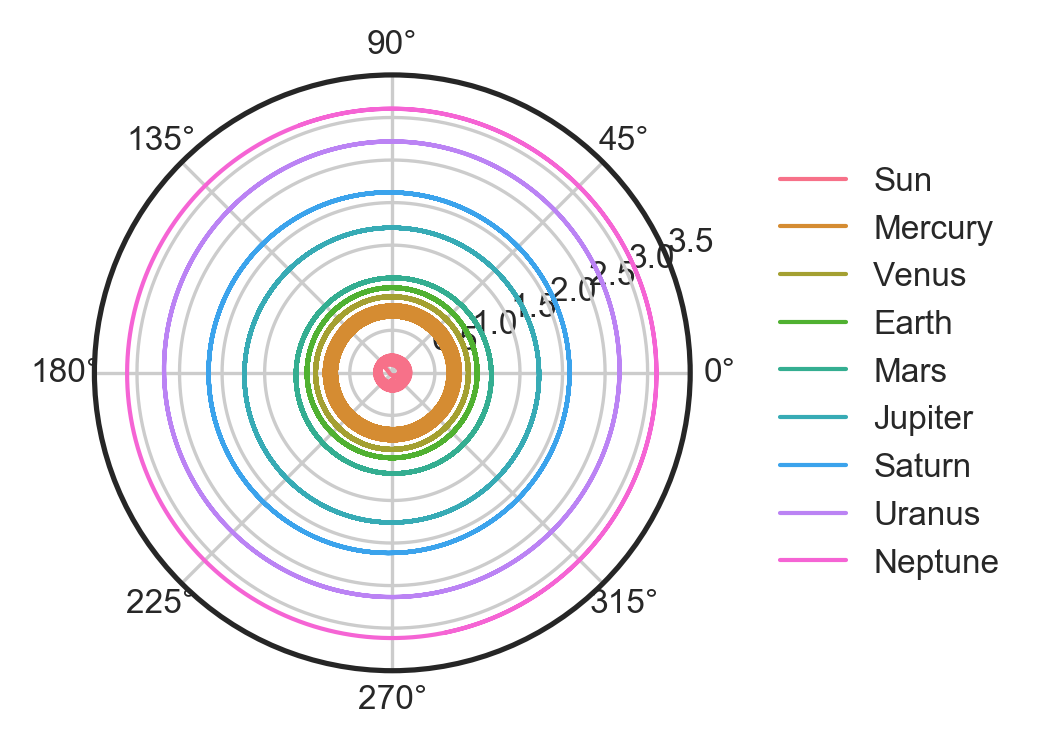
\includegraphics{planets_euler.png}
            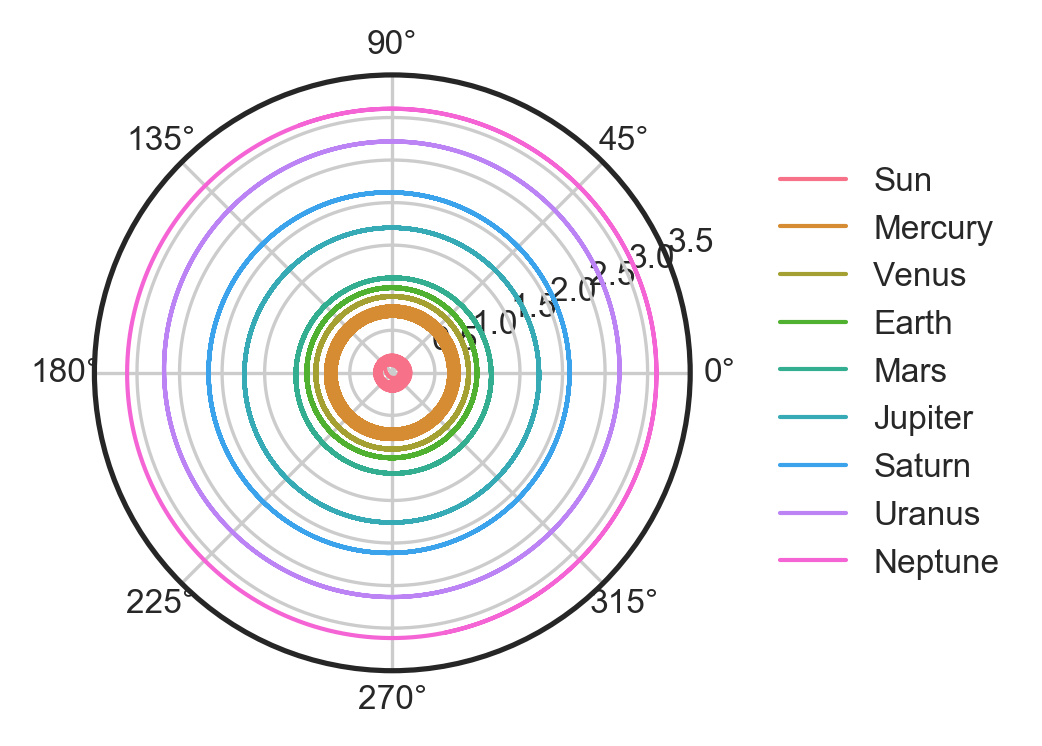
\includegraphics{planets_verlet.png}
            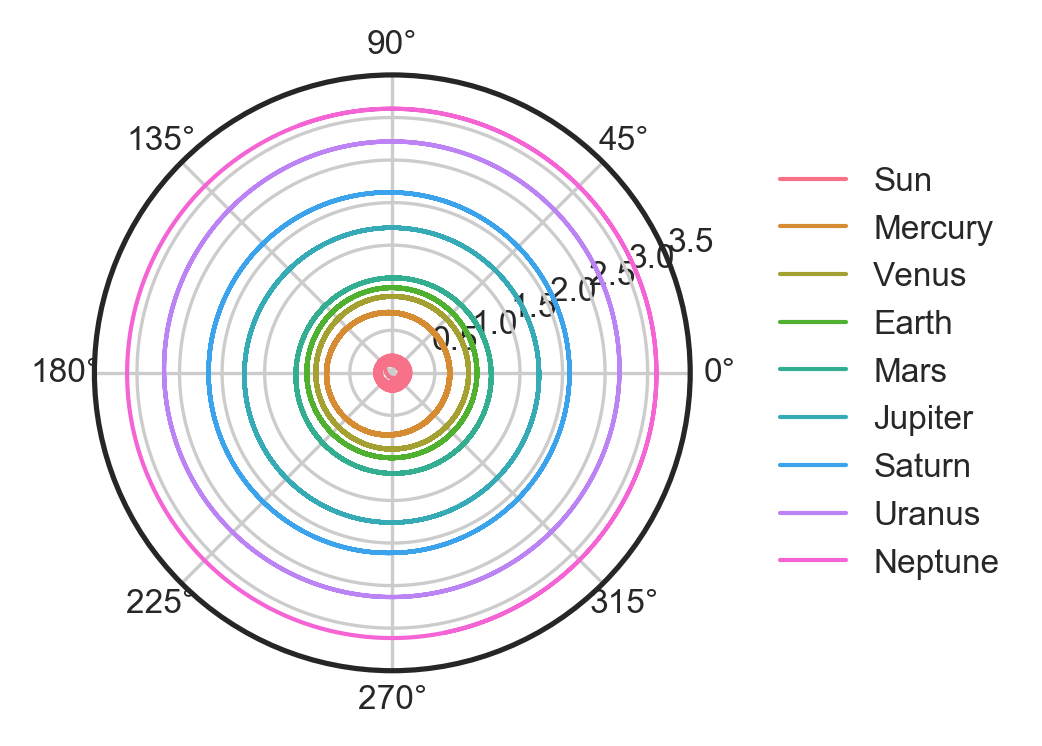
\includegraphics{planets_rk4.png}
            \caption{Orbits of Solar System bodies about the Solar System's barycenter, using the Euler (top), Verlet (middle) and RK4 (bottom) algorithms. The step size was \SI{1.0}{d} in each case, and the simulation ran for 91554 simulated days, which is longer than the orbital period of all of the planets. The radii are plotted as $\sqrt[3]{r}$ for better visibility of the inner planets. The orbits of the innermost planets (and especially Mercury) are unstable for the Euler and Verlet methods, but more stable for RK4.}
            \label{fig:system}
        \end{figure}





\end{document}
